\section{Data Analysis}

This analysis is performed using XENON100 Run-II science data, which corresponds to 224.9~live days. The detector response to
electronic recoil (ER) has been characterized using $^{60}$Co and $^{232}$Th radioactive sources, while response to inelastic nuclear recoil (NR)
scattering was calibrated using an $^{241}$AmBe source. 

The inelastic scattering of a WIMP with the nucleus of $^{129}$Xe produces an energy deposit via nuclear recoil with subsequent emission of  
a 39.6~KeV de-exitation photon. 
The largest fraction of the energy released in the event is via electronic recoil (ER) due to the emitted photon, this represents an
unusual signature for this kind of detector and brings the signal to overlay a phase space region with large backgrounds.
The choosen region of interest for this analysis surrounds the 39.6~KeV line in the cS1-cS2 plane which is further divided into
sub regions, as shown in figure~\ref{fig:SR}.

Events are asked, other than falling in the defined region of interest, to fullfill several selection criteria:
quality selection aimed to reduce noise impact toghether with energy and threshold selection on S2,
selection of single scatter events and fiducial volume definitions are reported in detail in \cite{dataAnalysis}, this analysis follows
the selection reported there for Run-II, only few modification have been designed specifically for this analysis and discussed below. 
In particular, selection on S2 width as a function of drift time has been optimized on a sample of events from 40~KeV of AmBe 
and set to a 95\% acceptance on those type of events. Events are required to be single scatter by applying a threshold on the 
second largest S2 peak size, in this analysis the threshold has been set to 160~PE and constant in S2 signal size. The fiducial
volume chosen for this analysis corresponds to 34~Kg of liquid xenon.


%brief explaination of the signature, selection cuts, few words about acceptances, image of signal region and control region.

\begin{figure}[h]
  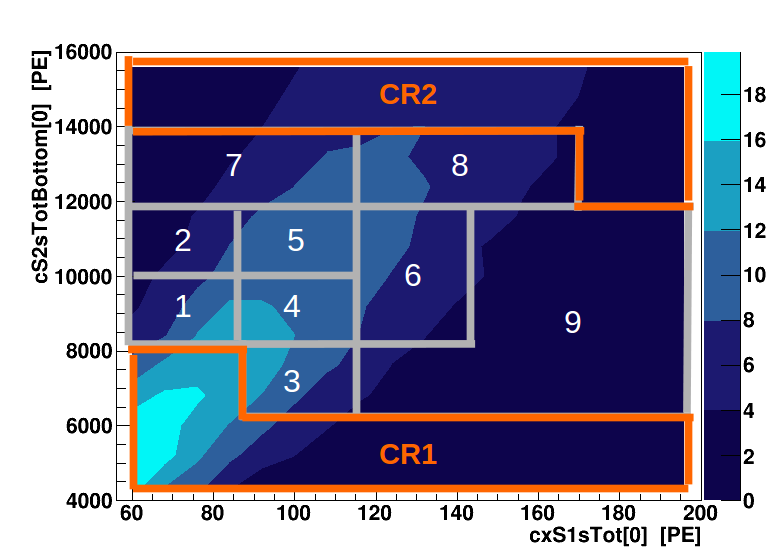
\includegraphics[width=\linewidth]{images/bkg_in_sr.png}
  \caption{Signal region and control region.}
  \label{fig:SR}
\end{figure}

\begin{figure}[h]
  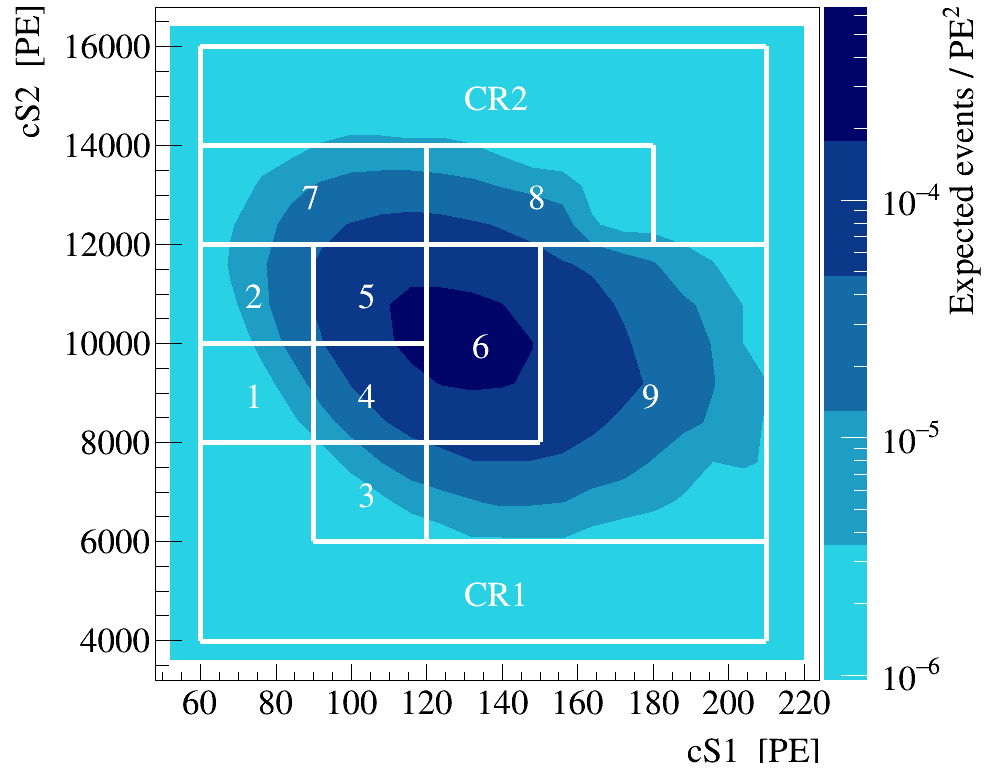
\includegraphics[width=\linewidth]{images/wimp_in_sr.png}
  \caption{Signal region and control region, for WIMP of mass 100~GeV.}
  \label{fig:SR2}
\end{figure}


\subsection{Signal Simulation} 
%description of the simulated signal, few words about cross checks MC matching.
The detector response to inelastic scattering of WIMPs of different masses off $^{129}$Xe nucleus was simulated using an empirical model.
The total deposited energy is divided into two independent contributions: the one related to the 39.6~KeV de-exitation photon and the one  relative to
the simultaneous nuclear recoil (NR) of the Xe atom, the number of photons and charge yield detected is simulated separatedly for each contribution
and then added togheter.

The electronic recoil (ER) induced by the de-exitation photon is produced 
The detector related light yield $L_y$ measured at 39.6~KeV with AmBe calibration has been found to have a large systematic uncertainty
due to the contribution of the nuclear recoil, so the light yield used to describe the number of photon detected is the result of a fit 
to data, corresponding to several lines, of the NEST model \cite{NEST,Geant1,Geant2}. The same model is used predict the charge yield at
39.6~KeV whichis then scaled according to the detector's secondary scintillation factor $Y$, determined from detector response to single electrons \cite{SingleE},
note that the corrected S2 observed by the bottom PMT array is used in this analysis. This is how the average $\mu_{cS1}$ and $\mu_{cS2}$ are obtained. 
The detector resolution at 39.6~KeV is embedded in three parameter the standard deviation in cS1 and cS2, respectively $\sigma_{cs1}$ and $\sigma_{cs2}$ and 
the correlation, $\rho$,  between cS1 and cS2. The correlation parameter is assumed to be independent of energy (at least in the considered range) and measured
using the 164~KeV Xenon activated line by AmBe calibration source, this line is choosen since allows to disentangle efficiently contribution from nuclear recoil,
the measured correlation is $\rho \, = \, -0.45 \pm 0.10$. Finally a two dimensional normal distribution, which is depicted in formula~\ref{f:2dgaus} except a normalization factor, 
is employed as a probability density function $f(cS1,cS2)$ distribution of energy deposited from the 39.6~KeV photon.
\begin{multline}
	f(cS1,cS2)  = exp \Big( -\frac{1}{2(1-\rho^2)} \Big[ \frac{(cS1 - \mu_{cS1})^2}{\sigma_{cs1}^2} + \\ 
	 \frac{(cS2 - \mu_{cS2})^2}{\sigma_{cs2}^2} - \frac{2\rho(cS1 - \mu_{cs1}) (cS2 - \mu_{cs2})} {\sigma_{cs1}\sigma_{cs2}} \Big] \Big) 
	%f(cS1,cS2) ~ = ~  \frac{1}{2 \pi \sigma_{cs1} \sigma_cs2 \sqrt{1-\rho^{2}} } exp \Big( -\frac{1}{2(1-\rho^2)} \Big[ \frac{(cS1 - \hat{cS1})^2}{\sigma_{cs1}^2} \Big] \Big)
\label{f:2dgaus}
\end{multline}


The cS1 and cS2 distributions from NR contribution to the total signal are predicted starting from the nuclear recoil energy spectrum
for inelastic interaction of a given WIMP mass \cite{inelastic_th}, the average cS1 and cS2 are given by formula~\ref{f:cs1} and~\ref{f:cs2} respectively,
where $\mathcal{L}_{eff}$ is the LXe relative scintillation efficiency while $S_{ee} \, = \, 0.58$  and $S_{nr} \, = \, 0.95$ describe the scintillation 
quenching due to the electric field \cite{ScintQuenching}. The parameterization and uncertainties of $\mathcal{L}_{eff}$ as a function of $E_{nr}$ are based on existing 
direct measurements \cite{run8Result}. The light yield at 122~keVee originate from the same NEST model fit as described above. For the cS2 the parameterization 
of $Q_{Y}(E_{nr})$ is taken from \cite{QY}.
all detector related resolution effects are introduced following the prescriptions described in \cite{dataAnalysis}.

\begin{equation}
cS1_{nr} ~=~ E_{nr} \, \mathcal{L}_{eff}(E_{nr}) \, L_{Y} \, \frac{S_{nr}}{S_{ee}}
\label{f:cs1}
\end{equation}

\begin{equation}
cS2_{nr}  ~ = ~ E_{nr} \, Q_{Y}(E_{nr}) \, Y
\label{f:cs2}
\end{equation}

The pdf of the ER and NR contributions are then convoluted toghether to obtain the overall pdf of the signal.
%The two contribution are summed toghether in an event-by-event basis using random extraction from the two pdfs. 
A 2D (cS1 versus cS2) acceptance map is applied to the signal pdf to reproduce data selection effects, single selection acceptances
are computed using calibration samples of AmBe for all the selection criteria except the outer volume veto and the single interaction selections, 
for which a detailed computation has been performed. The average acceptance value in the region of interest is of about $0.80 \pm 0.05$. 
An example of signal model is in Figure~\ref{fig:SR} for a WIMP of 100~GeV. 
The simulation of the 39.6~KeV line has been compared to AmBe data, for the comparison the proper AmBe nuclear recoil and acceptances
were simulated, the model was found in very well in agreement with calibration source data showing the largest discrepancies within 
statistical uncertainties.





\subsection {Background Model}

The expected background in the region of interest is mainly caused by material radioactivity, mainly photons that 
interact via compton scattering, background due to activation of Xe 39.6 line from radiogenic neutrons is found to be negligible.
To model this background we use data from $^{60}$Co calibration campaign, the assumption is
that the $^{60}$Co data are representative of the density in cS1-cS2 plane of the background. The calibration sample events
in the ROI amount to  22225 events, this yield is then scaled to data according to a measured background scale factor $\tau_{bkg}$.

The scale factor is measured in the two control regions shown in Figure~\ref{fig:SR} and labelled CR1 and CR2, the two control 
regions give compatible results and the computed average is $\tau_{bkg} \, =  \, 0.034 \pm 0.002 $, where the reported uncertainty 
is of statistical nature only.

The distribution of the calibration sample has been compared to the data of the sience run in the two control regions,
agreement is found within statistical uncertainties. $^{60}$Co calibration data have been compared in the region of interest to  
data from $^{232}$Th calibration campaign, the largest deviation between the two shapes is within 4\%. An additional systematic
uncertainty of 4\% has been applied to the expected background yield of each subregion of the ROI.












\subsection{Systematic Uncertainties}

few words, mainly a table summarizing uncertainties. Figure~\ref{fig:unc}.

\begin{figure}[h]
  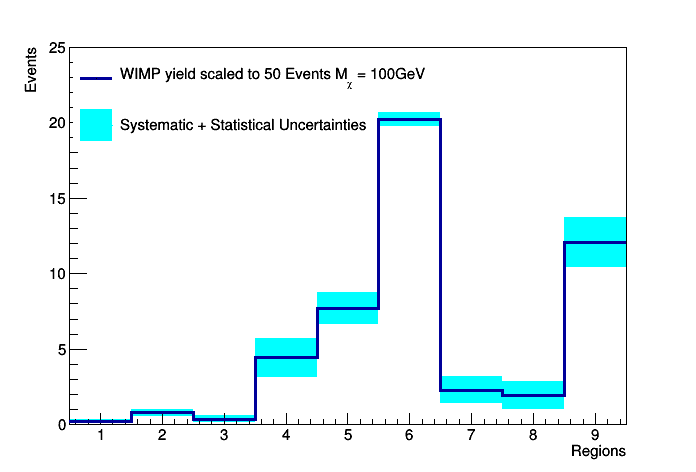
\includegraphics[width=\linewidth]{images/wimp_sys_unc.png}
  \caption{Signal region, uncertainties for WIMP of mass 100~GeV.}
  \label{fig:unc}
\end{figure}









